\documentclass[a4paper,10pt]{article}
\usepackage{listings}
\usepackage{color}
\usepackage{graphicx}
\usepackage{textcomp}

\lstset{language=Java}
\lstset{breaklines=true, numbers=left}
\lstset{tabsize=4}

\definecolor{CommentColor}{rgb}{0,0.5,0} 
\definecolor{KeywordColor}{rgb}{0,0,0.5}

\lstset{commentstyle=\scriptsize\color{CommentColor}\itshape}
\lstset{keywordstyle=\scriptsize\color{KeywordColor}\bfseries}
\lstset{basicstyle=\scriptsize}
\lstset{identifierstyle=\scriptsize}
\lstset{stringstyle=\scriptsize}

% \lstset{basicstyle=\ttfamily}

\definecolor{lightblue}{rgb}{0.7,0.7,1}
\definecolor{lightyellow}{rgb}{1,1,0.5}
\definecolor{lightred}{rgb}{1,0.5,0.5}
\definecolor{lightgreen}{rgb}{0.7,1,0.7}

\newcommand{\src}[1]{\texttt{#1}}

\newcommand{\property}[4]{\item[#1] \mbox{ } \begin{description} \item[Type] \src{#2} \item[Default] #3 \item[Usage] #4  \end{description}}

% thanks to http://www.alfredklomp.com/programming/tex/macros/
\long\def\greybox#1#2#3{%
    \newbox\contentbox%
    \newbox\bkgdbox%
    \setbox\contentbox\hbox to \hsize{%
        \vtop{
            \kern\columnsep
            \hbox to \hsize{%
                \kern\columnsep%
                \advance\hsize by -2\columnsep%
                \parbox{0.1\hsize}{\includegraphics[width=\hsize]{#2}}%
                \hspace{0.025\hsize}%
                \advance\hsize by -0.125\hsize%
                \setlength{\textwidth}{\hsize}%
                \vbox{
                    \parskip=\baselineskip
                    \parindent=0bp
                    \parbox[c]{\hsize}{#3}
                }%
                \kern\columnsep%
            }%
            \kern\columnsep%
        }%
    }%
    \setbox\bkgdbox\vbox{
	\color{#1}
        \hrule width  \wd\contentbox %
               height \ht\contentbox %
               depth  \dp\contentbox
	\color{black}
    }%
    \wd\bkgdbox=0bp%
    \vbox{\hbox to \hsize{\box\bkgdbox\box\contentbox}}%
    \vskip\baselineskip%
}

\newcommand{\designbox}[1]{\greybox{lightgreen}{design}{#1}}
\newcommand{\classbox}[1]{\greybox{lightyellow}{class}{#1}}
\newcommand{\warningbox}[1]{\greybox{lightred}{stop}{#1}}
\newcommand{\infobox}[1]{\greybox{lightblue}{info}{#1}}

\title{DockingFrames 1.0.8 - Core}
\author{Benjamin Sigg}

\begin{document}

\maketitle
\newpage

\tableofcontents
\newpage

\section{Drag and Drop}
Naturally, draging and droping of \src{Dockable}s is a key feature of the framework. Funny enough, the code actually involved in DnD is rather small compared to other modules of the framework.

\subsection{Relocator}
The sourcecode that detects drag gestures, searches for the target station and makes sure that the user has some visual feedback is located in the \linebreak \src{DefaultDockRelocator}. \src{DefaultDockRelocator} itself extends from \linebreak \src{DockRelocator} which just allows to register some listeners and set some useful properties.

\classbox{Clients seldomly need to implement their own \src{DockRelocator}. If they do, they have to implement a new \src{DockControllerFactory} in order to install their customized class. The method \src{createRelocator} is responsible for creating the new object.

This factory has then to be given to the constructor of a \src{DockController}.}

The \src{DockRelocator} that is in use can be accessed through the method \src{getRelocator} of \src{DockController}.

\subsection{Deciding what element to drag}
The \src{Relocator} needs to know where and when the user presses and moves the mouse. There are two solutions to this problem: either let the \src{Relocator} know what \src{Component}s are shown, or remotely control the \src{Relocator}. The first solution is achieved with \src{DockElementRepresentative}s, the second solution is achieved with the \src{RemoteRelocator}.

\subsubsection{DockElementRepresentative}
A \src{DockElementRepresentative} is a \src{Component} which represents a \src{Dockable}. Anyone can add \src{MouseInputListener}s to a representative and hence be informed about anything the mouse does on top of such a \src{Component}.

While the internal implementations of \src{DockElementRepresentative} are handled automatically by the framework, clients introducing new representatives will have to call the methods \src{addRepresentative} and \src{remoteRepresentative} of \src{DockController} to install or uninstall the item.

\infobox{\src{DockElementRepresentative} was added late to the framework. It carries some legacy code: the method \src{isUsedAsTitle}. This method introduces a distinction between those representations for which all features are activated (e.g. popup menus) and those for which only a selected subset is available. Normally clients implement representatives that are used as title and can return \src{true} here.}

\warningbox{The behavior for representations of \src{Dockable}s that are not registered is unspecified. Clients should not add a \src{DockElementRepresentative} if its \src{Dockable} is unknown to the \src{DockController}.}

\subsubsection{Remote control}
Sometimes it is not possible to implement a \src{DockElementRepresentative}. Remote control of a relocator is an alternative for these cases. Remote control is realized by the \src{RemoteRelocator}.

A \src{RemoteRelocator} can be optained by calling \src{createRemote} of \linebreak \src{DockRelocator}. \src{RemoteRelocator} should be used in combination with a \linebreak \src{MouseListener} and a \src{MouseMotionListener}:
\begin{itemize}
 \item \src{MouseListener.mousePressed} \textrightarrow \src{RemoteRelocator.init}
 \item \src{MouseMotionListener.mouseDragged} \textrightarrow \src{RemoteRelocator.drag}
 \item \src{MouseListener.mouseReleased} \textrightarrow \src{RemoteRelocator.drop}
\end{itemize}
The methods \src{init}, \src{drag} and \src{drop} return a \src{Reaction}. The reaction tells the caller what to do next:
\begin{itemize}
 \item \src{CONTINUE}: the operation continues, the event was ignored.
 \item \src{CONTINUE\_CONSUMED}: the operation continues, the event was consumed. The caller should invoke \src{MouseEvent.consume}.
 \item \src{BREAK}: the operation was canceled, the event was ignored.
 \item \src{BREAK\_CONSUMED}: the operation was canceled, the event was consumed. The caller should invoke \src{MouseEvent.consume}.
\end{itemize}

\classbox{There is a second interface called \src{DirectRemoteRelocator}. Instances can be optained by calling \src{createDirectRemote} of \src{DockRelocator}. A \src{DirectRemoteRelocator} is basically the same as a \src{RemoteRelocator} but always assumes that the user pressed the correct button on the mouse. Its methods do not return a \src{Reaction} because the event would always be consumed anyway.}

\infobox{Clients can use several remote controls at the same time, they will cancel out each other if necessary. A \src{RemoteRelocator} can be used several times.}

\subsection{Deciding where to drop an element}
A relocator needs to find the one \src{DockStation} on which the \src{Dockable} should be dropped. There is a default search algorithm which just orders all \src{DockStation}s by importance and visits them, and there are some interfaces which can influence the search.

\subsubsection{Search}
The \src{DefaultDockRelocator} searches the destination anew whenever the mouse is moved. A search consists of these steps::
\begin{enumerate}
 \item An ordered list of all potential destinations is built. A \src{DockStation} is a potential destination if it is visible (\src{isStationShowing} of \src{DockStation}), not the dragged \src{Dockable} nor one of its children. Each station offers a set of \src{DockStationDropLayer}s (\src{getLayers}), the layers decide whether the mouse is over a station or not. The order of the destinations depends on the priority of the layers, the parent-child relations between the stations and between the \src{Window}s on which the stations are.
 \item Then the method \src{prepareDrop} of \src{DockStation} is called. This method checks whether the station really is a good destination, if so it returns a \src{StationDropOperation}. The first station returning an operation is the destination.
 \item The method \src{draw} of the new operation is called, the method \src{destroy} on the old operation. The new operation will paint some markings to give a visual feedback to the user.
\end{enumerate}

\infobox{There is more information about the exact semantics in the API-documentation for \src{DockStation}.}

\classbox{Most of the work for drag and drop is done by the \src{DockStation}s themselfs, the \src{DockRelocator} just connects them. In order to complete the task the following methods and interfaces should be used:

\begin{itemize}
 \item \src{DockStation.accept} and \src{Dockable.accept} tells the station whether a child-parent relation is possible.
 \item \src{DockController.getAcceptance} allows access to the global \src{DockAcceptance}, an additional restriction that should be checked before allowing a drag and drop operation.
 \item To paint on the station, a \src{StationPaint} should be used. A \src{StationPaint} can be accessed through the \src{ThemeManager}.
\end{itemize}
}

\subsubsection{Drop}
Once the user releases the mouse, \src{Dockable} is dropped. The framework will call the method \src{execute} of \src{StationDropOperation}.

\begin{itemize}
 \item The \src{Dockable} may just be dropped aside of all the other children of the station. All that happens is that the \src{DockStation} gets a new child.
 \item The \src{Dockable} may be dropped over another child of the station. In this case the station may decide to combine the two children. The future parent \src{DockStation} will access a \src{Combiner} which defines how exactly two \src{Dockable}s can be merged into one, usually the answer is by creating a new \src{StackDockStation}. Clients can replace the current \src{Combiner} through the \src{ThemeManager}.
 \item If the dragged \src{Dockable} is a \src{DockStation} itself, it may be feasible to merge the parent and the new child \src{DockStation} into one station. The interface \src{Merger} is responsible for that. Clients can replace the default \src{Merger} by calling \src{DockRelocator.setMerger}.
\end{itemize}

\warningbox{Exchanging a \src{Combiner} or the \src{Merger} does not affect any existing \src{Dockable} or \src{DockStation}, it will only affect the creation of new elements.}

\subsection{Restrictions}
Not every possible \src{DockStation} is a good or valid target for a dragged \src{Dockable}. The framework applies a set of restrictions to drag and drop operations, these restrictions are implemented by ``acceptance tests''. Each acceptance test can veto against some child parent relations. The usual reasons why clients would want to implement their own tests consist of:
\begin{itemize}
 \item Some \src{Dockable} must always be visible.
 \item Some \src{DockStation}s represent a special area that can only be used by a subset of \src{Dockable}s.
 \item Some \src{Dockable}s can only be presented on a certain kind of \src{DockStation}.
\end{itemize}

Acceptance tests are performed during the drag and drop operation, but also if one of \src{DockStation.drop} methods is called. The acceptance tests are implemented by these methods:
\begin{itemize}
 \item Every \src{Dockable} has two methods called \src{accept}. One method checks whether the \src{Dockable} can be put directly onto some new parent, the other method checks whether the \src{Dockable} can be combined with an already existing child.
 \item Each \src{DockStation} has a method \src{accept}. This method tells whether some \src{Dockable} can become a child of the \src{DockStation}.
 \item And then there are \src{DockAcceptance}s. A \src{DockAcceptance} has \src{accept}-methods too. These methods get a \src{DockStation} and some \src{Dockable}s, and then have to decide whether the elements can be put together. Each \src{DockAcceptance} works on a global scale, and thus they are registered at the \src{DockController} through \src{addAcceptance}.
\end{itemize}

\warningbox{Acceptance tests are very powerful. They have to be implemented carefully or the drag and drop mechanism might become crippled.}

\designbox{Acceptance tests are performed by the potential destination \src{DockStation}. The \src{DockStation} is the first module that knows where a \src{Dockable} will land. Handling acceptance tests allows the station to cut down the amount of work it does, and to try alternative actions (e.g. a ``put'' instead of a ``merge'' action) if some future configuration does not pass the tests.

The drawback is, that a \src{DockStation} can break the mechanism by just not performing the tests.}

\subsection{Modes}
A \src{DockRelocator} can have "modes". A mode is some kind of behavior that is activated when the user presses a certain combination of keys. Modes are modeled by the class \src{DockRelocatorMode}. It is not specified what effect a mode really has, but normally a mode would add some restrictions where to put a \src{Dockable} during drag and drop. \src{DockRelocatorMode}s can be added or removed to a \src{DockRelocator} by the methods \src{addMode} and \src{removeMode}.

Currently two modes are installed:
\begin{description}
\item[DockRelocatorMode.SCREEN\_ONLY] (press key \textit{shift}) ensures that a \linebreak \src{Dockable} can only be put on a \src{ScreenDockStation}. That means that a \src{Dockable} can be directly above a \src{DockStation} like a \src{SplitDockStation}, but can't be dropped there.
\item[DockRelocatorMode.NO\_COMBINATION] (press key \textit{alt}) ensures that a \src{Dockable} can't be put over another \src{Dockable}. That means, every operation that would result in a merge is forbidden. Also dropping a \src{Dockable} on already merged \src{Dockable}s will not be allowed.
\end{description}

\classbox{The keys that have to be pressed to activate \src{SCREEN\_ONLY} or \src{NO\_COMBINATION} are the properties \src{SCREEN\_MASK} and \src{NO\_COMBINATION\_MASK}. The can be changed by accessing the \src{DockProperties}.}

\subsection{Animations}
During drag and drop, the framework may show some animations to help the user understand what effects dropping the \src{Dockable} would have. The animations usually involve moving or resizing the \src{Dockable}s that are not dragged. These animations are implemented with help of the \src{Span} interface. Each \src{Span} object represents some gap in the layout, a \src{Span} basically is a self mutating integer, to be understood as the size of a gap in pixels. Each \src{DockStation} may use several \src{Span}s at the same time, and an animation may involve multiple \src{Span}s changing their value simultaneously.

\infobox{ There are two sides involved in the animations:
\begin{itemize}
 \item The \src{DockStation}s define \emph{where} and \emph{when} the animations appear. For example a \src{FlapDockStation} can trigger an animation to insert empty space between each of its buttons.
 \item The \src{Span}s define \emph{how} an animation looks like. For example a \src{Span} could be implemented such that an animation starts slowly and increases its speed over time.
\end{itemize}}
Clients cannot tell a \src{DockStation} where the animations take place, but they can influence how the animations look like. To do that, clients need to implement both the \src{Span} and the \src{SpanFactory} interface. The \src{DockStation} will configure the \src{Span}, by associating different sizes (number of pixels) to different \src{SpanMode}s, and later by telling the \src{Span} which \src{SpanMode} currently is required. In return the \src{Span} will call the \src{resized} method of the \src{SpanCallback} whenever the size of the gap changes.

\classbox{To install a new \src{SpanFactory} clients can:
\begin{itemize}
 \item Use the property key \src{DockTheme.SPAN\_FACTORY} to globally change the factory.
 \item Use \src{ThemeManager.setSpanFactory} to change the factory only for one class of \src{DockStation}s.
 \item Calling \src{setSpanFactory} of \src{BasicTheme} \emph{before} the theme is installed.
\end{itemize}}
\warningbox{Some themes, like the \src{EclipseTheme}, deliberately disable the animations by installing the \src{NoSpanFactory}. }



\section{Drag and Drop}
Naturally, draging and droping of \src{Dockable}s is a key feature of the framework. Funny enough, the code actually involved in DnD is rather small compared to other modules of the framework.

\subsection{Relocator}
The sourcecode that detects drag gestures, searches for the target station and makes sure that the user has some visual feedback is located in the \linebreak \src{DefaultDockRelocator}. \src{DefaultDockRelocator} itself extends from \linebreak \src{DockRelocator} which just allows to register some listeners and set some useful properties.

\classbox{Clients seldomly need to implement their own \src{DockRelocator}. If they do, they have to implement a new \src{DockControllerFactory} in order to install their customized class. The method \src{createRelocator} is responsible for creating the new object.

This factory has then to be given to the constructor of a \src{DockController}.}

The \src{DockRelocator} that is in use can be accessed through the method \src{getRelocator} of \src{DockController}.

\subsection{Deciding what element to drag}
The \src{Relocator} needs to know where and when the user presses and moves the mouse. There are two solutions to this problem: either let the \src{Relocator} know what \src{Component}s are shown, or remotely control the \src{Relocator}. The first solution is achieved with \src{DockElementRepresentative}s, the second solution is achieved with the \src{RemoteRelocator}.

\subsubsection{DockElementRepresentative}
A \src{DockElementRepresentative} is a \src{Component} which represents a \src{Dockable}. Anyone can add \src{MouseInputListener}s to a representative and hence be informed about anything the mouse does on top of such a \src{Component}.

While the internal implementations of \src{DockElementRepresentative} are handled automatically by the framework, clients introducing new representatives will have to call the methods \src{addRepresentative} and \src{remoteRepresentative} of \src{DockController} to install or uninstall the item.

\infobox{\src{DockElementRepresentative} was added late to the framework. It carries some legacy code: the method \src{isUsedAsTitle}. This method introduces a distinction between those representations for which all features are activated (e.g. popup menus) and those for which only a selected subset is available. Normally clients implement representatives that are used as title and can return \src{true} here.}

\warningbox{The behavior for representations of \src{Dockable}s that are not registered is unspecified. Clients should not add a \src{DockElementRepresentative} if its \src{Dockable} is unknown to the \src{DockController}.}

\subsubsection{Remote control}
Sometimes it is not possible to implement a \src{DockElementRepresentative}. Remote control of a relocator is an alternative for these cases. Remote control is realized by the \src{RemoteRelocator}.

A \src{RemoteRelocator} can be optained by calling \src{createRemote} of \linebreak \src{DockRelocator}. \src{RemoteRelocator} should be used in combination with a \linebreak \src{MouseListener} and a \src{MouseMotionListener}:
\begin{itemize}
 \item \src{MouseListener.mousePressed} \textrightarrow \src{RemoteRelocator.init}
 \item \src{MouseMotionListener.mouseDragged} \textrightarrow \src{RemoteRelocator.drag}
 \item \src{MouseListener.mouseReleased} \textrightarrow \src{RemoteRelocator.drop}
\end{itemize}
The methods \src{init}, \src{drag} and \src{drop} return a \src{Reaction}. The reaction tells the caller what to do next:
\begin{itemize}
 \item \src{CONTINUE}: the operation continues, the event was ignored.
 \item \src{CONTINUE\_CONSUMED}: the operation continues, the event was consumed. The caller should invoke \src{MouseEvent.consume}.
 \item \src{BREAK}: the operation was canceled, the event was ignored.
 \item \src{BREAK\_CONSUMED}: the operation was canceled, the event was consumed. The caller should invoke \src{MouseEvent.consume}.
\end{itemize}

\classbox{There is a second interface called \src{DirectRemoteRelocator}. Instances can be optained by calling \src{createDirectRemote} of \src{DockRelocator}. A \src{DirectRemoteRelocator} is basically the same as a \src{RemoteRelocator} but always assumes that the user pressed the correct button on the mouse. Its methods do not return a \src{Reaction} because the event would always be consumed anyway.}

\infobox{Clients can use several remote controls at the same time, they will cancel out each other if necessary. A \src{RemoteRelocator} can be used several times.}

\subsection{Deciding where to drop an element}
A relocator needs to find the one \src{DockStation} on which the \src{Dockable} should be dropped. There is a default search algorithm which just orders all \src{DockStation}s by importance and visits them, and there are some interfaces which can influence the search.

\subsubsection{Search}
The \src{DefaultDockRelocator} searches the destination anew whenever the mouse is moved. A search consists of these steps::
\begin{enumerate}
 \item An ordered list of all potential destinations is built. A \src{DockStation} is a potential destination if it is visible (\src{isStationShowing} of \src{DockStation}), not the dragged \src{Dockable} nor one of its children. Each station offers a set of \src{DockStationDropLayer}s (\src{getLayers}), the layers decide whether the mouse is over a station or not. The order of the destinations depends on the priority of the layers, the parent-child relations between the stations and between the \src{Window}s on which the stations are.
 \item Then the method \src{prepareDrop} of \src{DockStation} is called. This method checks whether the station really is a good destination, if so it returns a \src{StationDropOperation}. The first station returning an operation is the destination.
 \item The method \src{draw} of the new operation is called, the method \src{destroy} on the old operation. The new operation will paint some markings to give a visual feedback to the user.
\end{enumerate}

\infobox{There is more information about the exact semantics in the API-documentation for \src{DockStation}.}

\classbox{Most of the work for drag and drop is done by the \src{DockStation}s themselfs, the \src{DockRelocator} just connects them. In order to complete the task the following methods and interfaces should be used:

\begin{itemize}
 \item \src{DockStation.accept} and \src{Dockable.accept} tells the station whether a child-parent relation is possible.
 \item \src{DockController.getAcceptance} allows access to the global \src{DockAcceptance}, an additional restriction that should be checked before allowing a drag and drop operation.
 \item To paint on the station, a \src{StationPaint} should be used. A \src{StationPaint} can be accessed through the \src{ThemeManager}.
\end{itemize}
}

\subsubsection{Drop}
Once the user releases the mouse, \src{Dockable} is dropped. The framework will call the method \src{execute} of \src{StationDropOperation}.

\begin{itemize}
 \item The \src{Dockable} may just be dropped aside of all the other children of the station. All that happens is that the \src{DockStation} gets a new child.
 \item The \src{Dockable} may be dropped over another child of the station. In this case the station may decide to combine the two children. The future parent \src{DockStation} will access a \src{Combiner} which defines how exactly two \src{Dockable}s can be merged into one, usually the answer is by creating a new \src{StackDockStation}. Clients can replace the current \src{Combiner} through the \src{ThemeManager}.
 \item If the dragged \src{Dockable} is a \src{DockStation} itself, it may be feasible to merge the parent and the new child \src{DockStation} into one station. The interface \src{Merger} is responsible for that. Clients can replace the default \src{Merger} by calling \src{DockRelocator.setMerger}.
\end{itemize}

\warningbox{Exchanging a \src{Combiner} or the \src{Merger} does not affect any existing \src{Dockable} or \src{DockStation}, it will only affect the creation of new elements.}

\subsection{Restrictions}
Not every possible \src{DockStation} is a good or valid target for a dragged \src{Dockable}. The framework applies a set of restrictions to drag and drop operations, these restrictions are implemented by ``acceptance tests''. Each acceptance test can veto against some child parent relations. The usual reasons why clients would want to implement their own tests consist of:
\begin{itemize}
 \item Some \src{Dockable} must always be visible.
 \item Some \src{DockStation}s represent a special area that can only be used by a subset of \src{Dockable}s.
 \item Some \src{Dockable}s can only be presented on a certain kind of \src{DockStation}.
\end{itemize}

Acceptance tests are performed during the drag and drop operation, but also if one of \src{DockStation.drop} methods is called. The acceptance tests are implemented by these methods:
\begin{itemize}
 \item Every \src{Dockable} has two methods called \src{accept}. One method checks whether the \src{Dockable} can be put directly onto some new parent, the other method checks whether the \src{Dockable} can be combined with an already existing child.
 \item Each \src{DockStation} has a method \src{accept}. This method tells whether some \src{Dockable} can become a child of the \src{DockStation}.
 \item And then there are \src{DockAcceptance}s. A \src{DockAcceptance} has \src{accept}-methods too. These methods get a \src{DockStation} and some \src{Dockable}s, and then have to decide whether the elements can be put together. Each \src{DockAcceptance} works on a global scale, and thus they are registered at the \src{DockController} through \src{addAcceptance}.
\end{itemize}

\warningbox{Acceptance tests are very powerful. They have to be implemented carefully or the drag and drop mechanism might become crippled.}

\designbox{Acceptance tests are performed by the potential destination \src{DockStation}. The \src{DockStation} is the first module that knows where a \src{Dockable} will land. Handling acceptance tests allows the station to cut down the amount of work it does, and to try alternative actions (e.g. a ``put'' instead of a ``merge'' action) if some future configuration does not pass the tests.

The drawback is, that a \src{DockStation} can break the mechanism by just not performing the tests.}

\subsection{Modes}
A \src{DockRelocator} can have "modes". A mode is some kind of behavior that is activated when the user presses a certain combination of keys. Modes are modeled by the class \src{DockRelocatorMode}. It is not specified what effect a mode really has, but normally a mode would add some restrictions where to put a \src{Dockable} during drag and drop. \src{DockRelocatorMode}s can be added or removed to a \src{DockRelocator} by the methods \src{addMode} and \src{removeMode}.

Currently two modes are installed:
\begin{description}
\item[DockRelocatorMode.SCREEN\_ONLY] (press key \textit{shift}) ensures that a \linebreak \src{Dockable} can only be put on a \src{ScreenDockStation}. That means that a \src{Dockable} can be directly above a \src{DockStation} like a \src{SplitDockStation}, but can't be dropped there.
\item[DockRelocatorMode.NO\_COMBINATION] (press key \textit{alt}) ensures that a \src{Dockable} can't be put over another \src{Dockable}. That means, every operation that would result in a merge is forbidden. Also dropping a \src{Dockable} on already merged \src{Dockable}s will not be allowed.
\end{description}

\classbox{The keys that have to be pressed to activate \src{SCREEN\_ONLY} or \src{NO\_COMBINATION} are the properties \src{SCREEN\_MASK} and \src{NO\_COMBINATION\_MASK}. The can be changed by accessing the \src{DockProperties}.}

\subsection{Animations}
During drag and drop, the framework may show some animations to help the user understand what effects dropping the \src{Dockable} would have. The animations usually involve moving or resizing the \src{Dockable}s that are not dragged. These animations are implemented with help of the \src{Span} interface. Each \src{Span} object represents some gap in the layout, a \src{Span} basically is a self mutating integer, to be understood as the size of a gap in pixels. Each \src{DockStation} may use several \src{Span}s at the same time, and an animation may involve multiple \src{Span}s changing their value simultaneously.

\infobox{ There are two sides involved in the animations:
\begin{itemize}
 \item The \src{DockStation}s define \emph{where} and \emph{when} the animations appear. For example a \src{FlapDockStation} can trigger an animation to insert empty space between each of its buttons.
 \item The \src{Span}s define \emph{how} an animation looks like. For example a \src{Span} could be implemented such that an animation starts slowly and increases its speed over time.
\end{itemize}}
Clients cannot tell a \src{DockStation} where the animations take place, but they can influence how the animations look like. To do that, clients need to implement both the \src{Span} and the \src{SpanFactory} interface. The \src{DockStation} will configure the \src{Span}, by associating different sizes (number of pixels) to different \src{SpanMode}s, and later by telling the \src{Span} which \src{SpanMode} currently is required. In return the \src{Span} will call the \src{resized} method of the \src{SpanCallback} whenever the size of the gap changes.

\classbox{To install a new \src{SpanFactory} clients can:
\begin{itemize}
 \item Use the property key \src{DockTheme.SPAN\_FACTORY} to globally change the factory.
 \item Use \src{ThemeManager.setSpanFactory} to change the factory only for one class of \src{DockStation}s.
 \item Calling \src{setSpanFactory} of \src{BasicTheme} \emph{before} the theme is installed.
\end{itemize}}
\warningbox{Some themes, like the \src{EclipseTheme}, deliberately disable the animations by installing the \src{NoSpanFactory}. }



\section{Drag and Drop}
Naturally, draging and droping of \src{Dockable}s is a key feature of the framework. Funny enough, the code actually involved in DnD is rather small compared to other modules of the framework.

\subsection{Relocator}
The sourcecode that detects drag gestures, searches for the target station and makes sure that the user has some visual feedback is located in the \linebreak \src{DefaultDockRelocator}. \src{DefaultDockRelocator} itself extends from \linebreak \src{DockRelocator} which just allows to register some listeners and set some useful properties.

\classbox{Clients seldomly need to implement their own \src{DockRelocator}. If they do, they have to implement a new \src{DockControllerFactory} in order to install their customized class. The method \src{createRelocator} is responsible for creating the new object.

This factory has then to be given to the constructor of a \src{DockController}.}

The \src{DockRelocator} that is in use can be accessed through the method \src{getRelocator} of \src{DockController}.

\subsection{Deciding what element to drag}
The \src{Relocator} needs to know where and when the user presses and moves the mouse. There are two solutions to this problem: either let the \src{Relocator} know what \src{Component}s are shown, or remotely control the \src{Relocator}. The first solution is achieved with \src{DockElementRepresentative}s, the second solution is achieved with the \src{RemoteRelocator}.

\subsubsection{DockElementRepresentative}
A \src{DockElementRepresentative} is a \src{Component} which represents a \src{Dockable}. Anyone can add \src{MouseInputListener}s to a representative and hence be informed about anything the mouse does on top of such a \src{Component}.

While the internal implementations of \src{DockElementRepresentative} are handled automatically by the framework, clients introducing new representatives will have to call the methods \src{addRepresentative} and \src{remoteRepresentative} of \src{DockController} to install or uninstall the item.

\infobox{\src{DockElementRepresentative} was added late to the framework. It carries some legacy code: the method \src{isUsedAsTitle}. This method introduces a distinction between those representations for which all features are activated (e.g. popup menus) and those for which only a selected subset is available. Normally clients implement representatives that are used as title and can return \src{true} here.}

\warningbox{The behavior for representations of \src{Dockable}s that are not registered is unspecified. Clients should not add a \src{DockElementRepresentative} if its \src{Dockable} is unknown to the \src{DockController}.}

\subsubsection{Remote control}
Sometimes it is not possible to implement a \src{DockElementRepresentative}. Remote control of a relocator is an alternative for these cases. Remote control is realized by the \src{RemoteRelocator}.

A \src{RemoteRelocator} can be optained by calling \src{createRemote} of \linebreak \src{DockRelocator}. \src{RemoteRelocator} should be used in combination with a \linebreak \src{MouseListener} and a \src{MouseMotionListener}:
\begin{itemize}
 \item \src{MouseListener.mousePressed} \textrightarrow \src{RemoteRelocator.init}
 \item \src{MouseMotionListener.mouseDragged} \textrightarrow \src{RemoteRelocator.drag}
 \item \src{MouseListener.mouseReleased} \textrightarrow \src{RemoteRelocator.drop}
\end{itemize}
The methods \src{init}, \src{drag} and \src{drop} return a \src{Reaction}. The reaction tells the caller what to do next:
\begin{itemize}
 \item \src{CONTINUE}: the operation continues, the event was ignored.
 \item \src{CONTINUE\_CONSUMED}: the operation continues, the event was consumed. The caller should invoke \src{MouseEvent.consume}.
 \item \src{BREAK}: the operation was canceled, the event was ignored.
 \item \src{BREAK\_CONSUMED}: the operation was canceled, the event was consumed. The caller should invoke \src{MouseEvent.consume}.
\end{itemize}

\classbox{There is a second interface called \src{DirectRemoteRelocator}. Instances can be optained by calling \src{createDirectRemote} of \src{DockRelocator}. A \src{DirectRemoteRelocator} is basically the same as a \src{RemoteRelocator} but always assumes that the user pressed the correct button on the mouse. Its methods do not return a \src{Reaction} because the event would always be consumed anyway.}

\infobox{Clients can use several remote controls at the same time, they will cancel out each other if necessary. A \src{RemoteRelocator} can be used several times.}

\subsection{Deciding where to drop an element}
A relocator needs to find the one \src{DockStation} on which the \src{Dockable} should be dropped. There is a default search algorithm which just orders all \src{DockStation}s by importance and visits them, and there are some interfaces which can influence the search.

\subsubsection{Search}
The \src{DefaultDockRelocator} searches the destination anew whenever the mouse is moved. A search consists of these steps::
\begin{enumerate}
 \item An ordered list of all potential destinations is built. A \src{DockStation} is a potential destination if it is visible (\src{isStationShowing} of \src{DockStation}), not the dragged \src{Dockable} nor one of its children. Each station offers a set of \src{DockStationDropLayer}s (\src{getLayers}), the layers decide whether the mouse is over a station or not. The order of the destinations depends on the priority of the layers, the parent-child relations between the stations and between the \src{Window}s on which the stations are.
 \item Then the method \src{prepareDrop} of \src{DockStation} is called. This method checks whether the station really is a good destination, if so it returns a \src{StationDropOperation}. The first station returning an operation is the destination.
 \item The method \src{draw} of the new operation is called, the method \src{destroy} on the old operation. The new operation will paint some markings to give a visual feedback to the user.
\end{enumerate}

\infobox{There is more information about the exact semantics in the API-documentation for \src{DockStation}.}

\classbox{Most of the work for drag and drop is done by the \src{DockStation}s themselfs, the \src{DockRelocator} just connects them. In order to complete the task the following methods and interfaces should be used:

\begin{itemize}
 \item \src{DockStation.accept} and \src{Dockable.accept} tells the station whether a child-parent relation is possible.
 \item \src{DockController.getAcceptance} allows access to the global \src{DockAcceptance}, an additional restriction that should be checked before allowing a drag and drop operation.
 \item To paint on the station, a \src{StationPaint} should be used. A \src{StationPaint} can be accessed through the \src{ThemeManager}.
\end{itemize}
}

\subsubsection{Drop}
Once the user releases the mouse, \src{Dockable} is dropped. The framework will call the method \src{execute} of \src{StationDropOperation}.

\begin{itemize}
 \item The \src{Dockable} may just be dropped aside of all the other children of the station. All that happens is that the \src{DockStation} gets a new child.
 \item The \src{Dockable} may be dropped over another child of the station. In this case the station may decide to combine the two children. The future parent \src{DockStation} will access a \src{Combiner} which defines how exactly two \src{Dockable}s can be merged into one, usually the answer is by creating a new \src{StackDockStation}. Clients can replace the current \src{Combiner} through the \src{ThemeManager}.
 \item If the dragged \src{Dockable} is a \src{DockStation} itself, it may be feasible to merge the parent and the new child \src{DockStation} into one station. The interface \src{Merger} is responsible for that. Clients can replace the default \src{Merger} by calling \src{DockRelocator.setMerger}.
\end{itemize}

\warningbox{Exchanging a \src{Combiner} or the \src{Merger} does not affect any existing \src{Dockable} or \src{DockStation}, it will only affect the creation of new elements.}

\subsection{Restrictions}
Not every possible \src{DockStation} is a good or valid target for a dragged \src{Dockable}. The framework applies a set of restrictions to drag and drop operations, these restrictions are implemented by ``acceptance tests''. Each acceptance test can veto against some child parent relations. The usual reasons why clients would want to implement their own tests consist of:
\begin{itemize}
 \item Some \src{Dockable} must always be visible.
 \item Some \src{DockStation}s represent a special area that can only be used by a subset of \src{Dockable}s.
 \item Some \src{Dockable}s can only be presented on a certain kind of \src{DockStation}.
\end{itemize}

Acceptance tests are performed during the drag and drop operation, but also if one of \src{DockStation.drop} methods is called. The acceptance tests are implemented by these methods:
\begin{itemize}
 \item Every \src{Dockable} has two methods called \src{accept}. One method checks whether the \src{Dockable} can be put directly onto some new parent, the other method checks whether the \src{Dockable} can be combined with an already existing child.
 \item Each \src{DockStation} has a method \src{accept}. This method tells whether some \src{Dockable} can become a child of the \src{DockStation}.
 \item And then there are \src{DockAcceptance}s. A \src{DockAcceptance} has \src{accept}-methods too. These methods get a \src{DockStation} and some \src{Dockable}s, and then have to decide whether the elements can be put together. Each \src{DockAcceptance} works on a global scale, and thus they are registered at the \src{DockController} through \src{addAcceptance}.
\end{itemize}

\warningbox{Acceptance tests are very powerful. They have to be implemented carefully or the drag and drop mechanism might become crippled.}

\designbox{Acceptance tests are performed by the potential destination \src{DockStation}. The \src{DockStation} is the first module that knows where a \src{Dockable} will land. Handling acceptance tests allows the station to cut down the amount of work it does, and to try alternative actions (e.g. a ``put'' instead of a ``merge'' action) if some future configuration does not pass the tests.

The drawback is, that a \src{DockStation} can break the mechanism by just not performing the tests.}

\subsection{Modes}
A \src{DockRelocator} can have "modes". A mode is some kind of behavior that is activated when the user presses a certain combination of keys. Modes are modeled by the class \src{DockRelocatorMode}. It is not specified what effect a mode really has, but normally a mode would add some restrictions where to put a \src{Dockable} during drag and drop. \src{DockRelocatorMode}s can be added or removed to a \src{DockRelocator} by the methods \src{addMode} and \src{removeMode}.

Currently two modes are installed:
\begin{description}
\item[DockRelocatorMode.SCREEN\_ONLY] (press key \textit{shift}) ensures that a \linebreak \src{Dockable} can only be put on a \src{ScreenDockStation}. That means that a \src{Dockable} can be directly above a \src{DockStation} like a \src{SplitDockStation}, but can't be dropped there.
\item[DockRelocatorMode.NO\_COMBINATION] (press key \textit{alt}) ensures that a \src{Dockable} can't be put over another \src{Dockable}. That means, every operation that would result in a merge is forbidden. Also dropping a \src{Dockable} on already merged \src{Dockable}s will not be allowed.
\end{description}

\classbox{The keys that have to be pressed to activate \src{SCREEN\_ONLY} or \src{NO\_COMBINATION} are the properties \src{SCREEN\_MASK} and \src{NO\_COMBINATION\_MASK}. The can be changed by accessing the \src{DockProperties}.}

\subsection{Animations}
During drag and drop, the framework may show some animations to help the user understand what effects dropping the \src{Dockable} would have. The animations usually involve moving or resizing the \src{Dockable}s that are not dragged. These animations are implemented with help of the \src{Span} interface. Each \src{Span} object represents some gap in the layout, a \src{Span} basically is a self mutating integer, to be understood as the size of a gap in pixels. Each \src{DockStation} may use several \src{Span}s at the same time, and an animation may involve multiple \src{Span}s changing their value simultaneously.

\infobox{ There are two sides involved in the animations:
\begin{itemize}
 \item The \src{DockStation}s define \emph{where} and \emph{when} the animations appear. For example a \src{FlapDockStation} can trigger an animation to insert empty space between each of its buttons.
 \item The \src{Span}s define \emph{how} an animation looks like. For example a \src{Span} could be implemented such that an animation starts slowly and increases its speed over time.
\end{itemize}}
Clients cannot tell a \src{DockStation} where the animations take place, but they can influence how the animations look like. To do that, clients need to implement both the \src{Span} and the \src{SpanFactory} interface. The \src{DockStation} will configure the \src{Span}, by associating different sizes (number of pixels) to different \src{SpanMode}s, and later by telling the \src{Span} which \src{SpanMode} currently is required. In return the \src{Span} will call the \src{resized} method of the \src{SpanCallback} whenever the size of the gap changes.

\classbox{To install a new \src{SpanFactory} clients can:
\begin{itemize}
 \item Use the property key \src{DockTheme.SPAN\_FACTORY} to globally change the factory.
 \item Use \src{ThemeManager.setSpanFactory} to change the factory only for one class of \src{DockStation}s.
 \item Calling \src{setSpanFactory} of \src{BasicTheme} \emph{before} the theme is installed.
\end{itemize}}
\warningbox{Some themes, like the \src{EclipseTheme}, deliberately disable the animations by installing the \src{NoSpanFactory}. }



\section{Drag and Drop}
Naturally, draging and droping of \src{Dockable}s is a key feature of the framework. Funny enough, the code actually involved in DnD is rather small compared to other modules of the framework.

\subsection{Relocator}
The sourcecode that detects drag gestures, searches for the target station and makes sure that the user has some visual feedback is located in the \linebreak \src{DefaultDockRelocator}. \src{DefaultDockRelocator} itself extends from \linebreak \src{DockRelocator} which just allows to register some listeners and set some useful properties.

\classbox{Clients seldomly need to implement their own \src{DockRelocator}. If they do, they have to implement a new \src{DockControllerFactory} in order to install their customized class. The method \src{createRelocator} is responsible for creating the new object.

This factory has then to be given to the constructor of a \src{DockController}.}

The \src{DockRelocator} that is in use can be accessed through the method \src{getRelocator} of \src{DockController}.

\subsection{Deciding what element to drag}
The \src{Relocator} needs to know where and when the user presses and moves the mouse. There are two solutions to this problem: either let the \src{Relocator} know what \src{Component}s are shown, or remotely control the \src{Relocator}. The first solution is achieved with \src{DockElementRepresentative}s, the second solution is achieved with the \src{RemoteRelocator}.

\subsubsection{DockElementRepresentative}
A \src{DockElementRepresentative} is a \src{Component} which represents a \src{Dockable}. Anyone can add \src{MouseInputListener}s to a representative and hence be informed about anything the mouse does on top of such a \src{Component}.

While the internal implementations of \src{DockElementRepresentative} are handled automatically by the framework, clients introducing new representatives will have to call the methods \src{addRepresentative} and \src{remoteRepresentative} of \src{DockController} to install or uninstall the item.

\infobox{\src{DockElementRepresentative} was added late to the framework. It carries some legacy code: the method \src{isUsedAsTitle}. This method introduces a distinction between those representations for which all features are activated (e.g. popup menus) and those for which only a selected subset is available. Normally clients implement representatives that are used as title and can return \src{true} here.}

\warningbox{The behavior for representations of \src{Dockable}s that are not registered is unspecified. Clients should not add a \src{DockElementRepresentative} if its \src{Dockable} is unknown to the \src{DockController}.}

\subsubsection{Remote control}
Sometimes it is not possible to implement a \src{DockElementRepresentative}. Remote control of a relocator is an alternative for these cases. Remote control is realized by the \src{RemoteRelocator}.

A \src{RemoteRelocator} can be optained by calling \src{createRemote} of \linebreak \src{DockRelocator}. \src{RemoteRelocator} should be used in combination with a \linebreak \src{MouseListener} and a \src{MouseMotionListener}:
\begin{itemize}
 \item \src{MouseListener.mousePressed} \textrightarrow \src{RemoteRelocator.init}
 \item \src{MouseMotionListener.mouseDragged} \textrightarrow \src{RemoteRelocator.drag}
 \item \src{MouseListener.mouseReleased} \textrightarrow \src{RemoteRelocator.drop}
\end{itemize}
The methods \src{init}, \src{drag} and \src{drop} return a \src{Reaction}. The reaction tells the caller what to do next:
\begin{itemize}
 \item \src{CONTINUE}: the operation continues, the event was ignored.
 \item \src{CONTINUE\_CONSUMED}: the operation continues, the event was consumed. The caller should invoke \src{MouseEvent.consume}.
 \item \src{BREAK}: the operation was canceled, the event was ignored.
 \item \src{BREAK\_CONSUMED}: the operation was canceled, the event was consumed. The caller should invoke \src{MouseEvent.consume}.
\end{itemize}

\classbox{There is a second interface called \src{DirectRemoteRelocator}. Instances can be optained by calling \src{createDirectRemote} of \src{DockRelocator}. A \src{DirectRemoteRelocator} is basically the same as a \src{RemoteRelocator} but always assumes that the user pressed the correct button on the mouse. Its methods do not return a \src{Reaction} because the event would always be consumed anyway.}

\infobox{Clients can use several remote controls at the same time, they will cancel out each other if necessary. A \src{RemoteRelocator} can be used several times.}

\subsection{Deciding where to drop an element}
A relocator needs to find the one \src{DockStation} on which the \src{Dockable} should be dropped. There is a default search algorithm which just orders all \src{DockStation}s by importance and visits them, and there are some interfaces which can influence the search.

\subsubsection{Search}
The \src{DefaultDockRelocator} searches the destination anew whenever the mouse is moved. A search consists of these steps::
\begin{enumerate}
 \item An ordered list of all potential destinations is built. A \src{DockStation} is a potential destination if it is visible (\src{isStationShowing} of \src{DockStation}), not the dragged \src{Dockable} nor one of its children. Each station offers a set of \src{DockStationDropLayer}s (\src{getLayers}), the layers decide whether the mouse is over a station or not. The order of the destinations depends on the priority of the layers, the parent-child relations between the stations and between the \src{Window}s on which the stations are.
 \item Then the method \src{prepareDrop} of \src{DockStation} is called. This method checks whether the station really is a good destination, if so it returns a \src{StationDropOperation}. The first station returning an operation is the destination.
 \item The method \src{draw} of the new operation is called, the method \src{destroy} on the old operation. The new operation will paint some markings to give a visual feedback to the user.
\end{enumerate}

\infobox{There is more information about the exact semantics in the API-documentation for \src{DockStation}.}

\classbox{Most of the work for drag and drop is done by the \src{DockStation}s themselfs, the \src{DockRelocator} just connects them. In order to complete the task the following methods and interfaces should be used:

\begin{itemize}
 \item \src{DockStation.accept} and \src{Dockable.accept} tells the station whether a child-parent relation is possible.
 \item \src{DockController.getAcceptance} allows access to the global \src{DockAcceptance}, an additional restriction that should be checked before allowing a drag and drop operation.
 \item To paint on the station, a \src{StationPaint} should be used. A \src{StationPaint} can be accessed through the \src{ThemeManager}.
\end{itemize}
}

\subsubsection{Drop}
Once the user releases the mouse, \src{Dockable} is dropped. The framework will call the method \src{execute} of \src{StationDropOperation}.

\begin{itemize}
 \item The \src{Dockable} may just be dropped aside of all the other children of the station. All that happens is that the \src{DockStation} gets a new child.
 \item The \src{Dockable} may be dropped over another child of the station. In this case the station may decide to combine the two children. The future parent \src{DockStation} will access a \src{Combiner} which defines how exactly two \src{Dockable}s can be merged into one, usually the answer is by creating a new \src{StackDockStation}. Clients can replace the current \src{Combiner} through the \src{ThemeManager}.
 \item If the dragged \src{Dockable} is a \src{DockStation} itself, it may be feasible to merge the parent and the new child \src{DockStation} into one station. The interface \src{Merger} is responsible for that. Clients can replace the default \src{Merger} by calling \src{DockRelocator.setMerger}.
\end{itemize}

\warningbox{Exchanging a \src{Combiner} or the \src{Merger} does not affect any existing \src{Dockable} or \src{DockStation}, it will only affect the creation of new elements.}

\subsection{Restrictions}
Not every possible \src{DockStation} is a good or valid target for a dragged \src{Dockable}. The framework applies a set of restrictions to drag and drop operations, these restrictions are implemented by ``acceptance tests''. Each acceptance test can veto against some child parent relations. The usual reasons why clients would want to implement their own tests consist of:
\begin{itemize}
 \item Some \src{Dockable} must always be visible.
 \item Some \src{DockStation}s represent a special area that can only be used by a subset of \src{Dockable}s.
 \item Some \src{Dockable}s can only be presented on a certain kind of \src{DockStation}.
\end{itemize}

Acceptance tests are performed during the drag and drop operation, but also if one of \src{DockStation.drop} methods is called. The acceptance tests are implemented by these methods:
\begin{itemize}
 \item Every \src{Dockable} has two methods called \src{accept}. One method checks whether the \src{Dockable} can be put directly onto some new parent, the other method checks whether the \src{Dockable} can be combined with an already existing child.
 \item Each \src{DockStation} has a method \src{accept}. This method tells whether some \src{Dockable} can become a child of the \src{DockStation}.
 \item And then there are \src{DockAcceptance}s. A \src{DockAcceptance} has \src{accept}-methods too. These methods get a \src{DockStation} and some \src{Dockable}s, and then have to decide whether the elements can be put together. Each \src{DockAcceptance} works on a global scale, and thus they are registered at the \src{DockController} through \src{addAcceptance}.
\end{itemize}

\warningbox{Acceptance tests are very powerful. They have to be implemented carefully or the drag and drop mechanism might become crippled.}

\designbox{Acceptance tests are performed by the potential destination \src{DockStation}. The \src{DockStation} is the first module that knows where a \src{Dockable} will land. Handling acceptance tests allows the station to cut down the amount of work it does, and to try alternative actions (e.g. a ``put'' instead of a ``merge'' action) if some future configuration does not pass the tests.

The drawback is, that a \src{DockStation} can break the mechanism by just not performing the tests.}

\subsection{Modes}
A \src{DockRelocator} can have "modes". A mode is some kind of behavior that is activated when the user presses a certain combination of keys. Modes are modeled by the class \src{DockRelocatorMode}. It is not specified what effect a mode really has, but normally a mode would add some restrictions where to put a \src{Dockable} during drag and drop. \src{DockRelocatorMode}s can be added or removed to a \src{DockRelocator} by the methods \src{addMode} and \src{removeMode}.

Currently two modes are installed:
\begin{description}
\item[DockRelocatorMode.SCREEN\_ONLY] (press key \textit{shift}) ensures that a \linebreak \src{Dockable} can only be put on a \src{ScreenDockStation}. That means that a \src{Dockable} can be directly above a \src{DockStation} like a \src{SplitDockStation}, but can't be dropped there.
\item[DockRelocatorMode.NO\_COMBINATION] (press key \textit{alt}) ensures that a \src{Dockable} can't be put over another \src{Dockable}. That means, every operation that would result in a merge is forbidden. Also dropping a \src{Dockable} on already merged \src{Dockable}s will not be allowed.
\end{description}

\classbox{The keys that have to be pressed to activate \src{SCREEN\_ONLY} or \src{NO\_COMBINATION} are the properties \src{SCREEN\_MASK} and \src{NO\_COMBINATION\_MASK}. The can be changed by accessing the \src{DockProperties}.}

\subsection{Animations}
During drag and drop, the framework may show some animations to help the user understand what effects dropping the \src{Dockable} would have. The animations usually involve moving or resizing the \src{Dockable}s that are not dragged. These animations are implemented with help of the \src{Span} interface. Each \src{Span} object represents some gap in the layout, a \src{Span} basically is a self mutating integer, to be understood as the size of a gap in pixels. Each \src{DockStation} may use several \src{Span}s at the same time, and an animation may involve multiple \src{Span}s changing their value simultaneously.

\infobox{ There are two sides involved in the animations:
\begin{itemize}
 \item The \src{DockStation}s define \emph{where} and \emph{when} the animations appear. For example a \src{FlapDockStation} can trigger an animation to insert empty space between each of its buttons.
 \item The \src{Span}s define \emph{how} an animation looks like. For example a \src{Span} could be implemented such that an animation starts slowly and increases its speed over time.
\end{itemize}}
Clients cannot tell a \src{DockStation} where the animations take place, but they can influence how the animations look like. To do that, clients need to implement both the \src{Span} and the \src{SpanFactory} interface. The \src{DockStation} will configure the \src{Span}, by associating different sizes (number of pixels) to different \src{SpanMode}s, and later by telling the \src{Span} which \src{SpanMode} currently is required. In return the \src{Span} will call the \src{resized} method of the \src{SpanCallback} whenever the size of the gap changes.

\classbox{To install a new \src{SpanFactory} clients can:
\begin{itemize}
 \item Use the property key \src{DockTheme.SPAN\_FACTORY} to globally change the factory.
 \item Use \src{ThemeManager.setSpanFactory} to change the factory only for one class of \src{DockStation}s.
 \item Calling \src{setSpanFactory} of \src{BasicTheme} \emph{before} the theme is installed.
\end{itemize}}
\warningbox{Some themes, like the \src{EclipseTheme}, deliberately disable the animations by installing the \src{NoSpanFactory}. }



\section{Titles} \label{sec:titles}
A \src{DockTitle} is a \src{Component} that may show an icon, a text, some \src{DockAction}s or other information about a \src{Dockable}. Users often grab a \src{DockTitle} when they want to start a drag \& drop operation.

\begin{figure}[h]
\centering
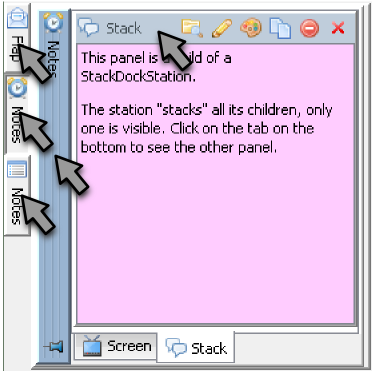
\includegraphics[scale=0.5]{titles}
\caption{Some \src{DockTitles}.}
\label{fig:titles}
\end{figure}

\subsection{Lifecycle}
Any client that wants to show a \src{DockTitle} needs to specify what \textit{kind} of title it shows and needs to \textit{request} a title.

The \textit{kind} of a title is specified by a \src{DockTitleVersion}. New \linebreak \src{DockTitleVersion}s are obtained through the \src{DockTitleManager} (there is one per \src{DockController}). Creating a new \src{DockTitleVersion} requires the calling client to provide a default \src{DockTitleFactory}.

The \textit{request} for a title is handled by a \src{DockTitleRequest}. Once a \linebreak \src{DockTitleRequest} is created its method \src{request} can be called to execute the request. Clients should call \src{install} before using the request and \src{uninstall} once the request is no longer in use. This way the \src{DockTitleRequest} will automatically be executed again if the underlying \src{DockTitleFactory} is exchanged.

Once a \src{DockTitle} is acquired it must be connected with its \src{Dockable}. Clients must call the method \src{bind( DockTitle )} of \src{Dockable}, this tells the \src{Dockable} that is has a new title. If the client no longer shows the title it must call \src{unbind( DockTitle )}.

\warningbox{Do not call the method \src{bind} or \src{unbind} of \src{DockTitle}, these methods are called automatically by the \src{DockController}.}

\infobox{\src{Dockable}s provide some information about their titles:
\begin{itemize}
	\item The method \src{listBoundTitles} returns an list of all \src{DockTitle}s which are currently in use for the \src{Dockable}.
	\item A \src{DockableListener} has several methods that will be invoked if titles get added, removed, updated or exchanged.
\end{itemize}}

\subsection{Custom titles}
\subsubsection{Implementing a new title}
It is possible to replace all the titles in the framework. While the interface \src{DockTitle} is rather open, a title is responsible to collect all the information it wants to show by itself.

Most titles will have a constructor that has a \src{Dockable} as argument. They will add a \src{DockableListener} to their \src{Dockable} once \src{bind} is called and remove the listener once \src{unbind} is called.

There is only one connection between a module that shows a title and the title itself: the method \src{changed}. Modules use this method to send \linebreak \src{DockTitleEvent}s to the title.

\designbox{A module does not need to know what title it shows. It just delivers the \src{DockTitleEvent} to the title. The module can use a subclass of \src{DockTitleEvent} to transfer more information than \src{DockTitleEvent} alone could carry. This design allows to use any implementation of \src{DockTitle} at any place while some titles still can use additional information from their environment. An example is the \src{EclipseDockTitleEvent} which is used by tabs. This event also tells the titles at which location they are and whether their tab is focused or not.}

There are some classes that can help implementing a custom title:
\begin{itemize}
	\item \src{AbstractDockTitle} provides standard implementations for most of the features a title requires. Subclasses only need to override the method \linebreak \src{paintBackground} to have their custom painting code used.
	\item \src{BasicDockTitle} paints some gradients as background. Clients can change the color of these gradients. This title is also a good reference of how things can be done.
	\item \src{ButtonPanel} is a \src{Component} able to display a set of \src{DockAction}s. \linebreak \src{ButtonPanel} is able to show a popup-menu if there is not enough space for all actions.
\end{itemize}

\classbox{In order to use the popup menu of \src{ButtonPanel} some special code has to be written. First: the argument \src{menu} of the constructor of \src{ButtonPanel} has to be set to \src{true}. Second: the method \src{getPreferredSize} of \src{ButtonPanel} cannot be used, any standard \src{LayoutManager} will fail. Instead the method \src{doLayout} of the \src{Container} which shows the panel can be overriden. In this \src{doLayout} method the container should call \src{getPreferredSizes} to obtain a list of possible sizes of the panel. The $n$'th dimension in this array tells how big the \src{ButtonPanel} would be if it would show $n$ actions. The container should choose the biggest possible $n$ and call \src{setVisibleActions}.}

\subsubsection{Apply the title}
There are several ways to introduce a custom title into the framework.

To override or implement \src{requestDockTitle} of \src{Dockable} is the simplest way. The method just creates a new instance of the custom title when called.

Overriding or implementing \src{requestChildDockTitle} of \src{DockStation} allows to exchange the title of all children.

The \src{DockTheme} can be used as well. Either override the method \linebreak \src{getTitleFactory} or call \src{setTitleFactory} when using a \src{BasicTheme}. With a few exceptions all the modules use the factory of the theme, hence replacing this factory will have a big effect.

Or use the \src{DockTitleManager} to make some better tuned settings. The \linebreak \src{DockTitleManager} can be accessed by calling \src{getDockTitleManager} of \linebreak \src{DockController}. Search the unique string identifier of the module that uses a title and call \src{getVersion} to access the associated \src{DockTitleVersion}. Then with the help of \src{setFactory} a new factory can be introduced. In code this could look like this:
\begin{lstlisting}
DockController controller = ...

DockTitleManager manager = controller.getDockTitleManager();
DockTitleVersion version =
  manager.getVersion( SplitDockStation.TITLE_ID, null );
version.setFactory( new CustomDockTitleFactory(), Priority.CLIENT );
\end{lstlisting}

\section{Themes}
A \src{DockTheme} relates to \src{DockingFrames} like a \src{LookAndFeel} to \src{Java Swing}. At any given time a \src{DockController} is associated with exactly one theme. The theme defines various graphical elements like icons, painting code and also some behavior. The current \src{DockTheme} can be changed through the method \src{setTheme}:
\begin{lstlisting}
DockController controller = ...
DockTheme theme = new EclipseTheme();
controller.setTheme( theme );
\end{lstlisting}

\subsection{Existing Themes}
Several \src{DockTheme}s are already included in the framework. A list of theme-factories can be accessed through the method \src{getThemes} of \src{DockUI}. This sub-chapter will list up the existing themes and mention some of their specialities.

Keep in mind that \src{DockTheme}s do not have to follow a specific path for setting up their views. All the current themes are derived from \src{BasicTheme} and thus share a lot of concepts. Future or custom themes however might be implemented in different ways.

\subsubsection{NoStackTheme}
This theme is a wrapper around other themes. It prevents \src{StackDockStation}s from having a \src{DockTitle} and makes sure that the user cannot drag or create a \src{StackDockStation} into another \src{StackDockStation}. The code for creating a \src{NoStackTheme} looks like this:
\begin{lstlisting}
DockTheme original = ...
DockTheme theme = new NoStackTheme( original );
\end{lstlisting}

\subsubsection{BasicTheme}
The \src{BasicTheme} is a simple but working theme. All the other themes of the framework build upon \src{BasicTheme}. This theme shows content whenever possible. It tries to use all features and thus is quite good for debugging, to check whether all features are supported.

\begin{figure}[ht]
\centering
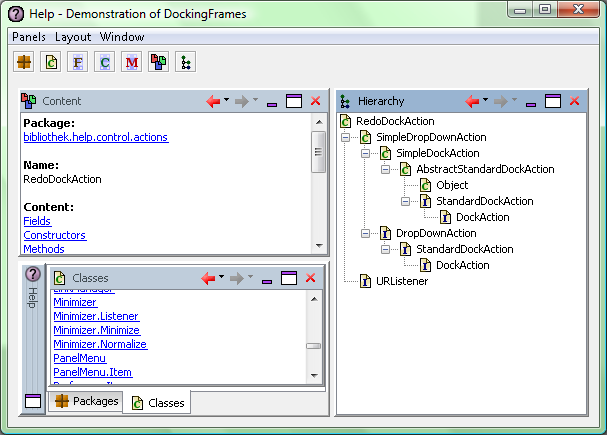
\includegraphics[width=0.5\textwidth]{theme_default}
\caption{BasicTheme}
\label{fig:theme_flat}
\end{figure}

\subsubsection{SmoothTheme}
\src{SmoothTheme} is basically the same as \src{BasicTheme}. The only difference is a replaced default-\src{DockTitleFactory}. As a result new \src{DockTitle}s are used by most elements, these new titles smoothly change their color when the ``active'' state of their \src{Dockable}s changes.

\subsubsection{FlatTheme}
\src{FlatTheme} is a variation of \src{BasicTheme} that tries to minimze the number of borders. Among other things it uses new \src{DockTitle}s and new views for \src{DockAction}s. It is the ideal theme for developers that want to learn how to customize an existing theme.

\begin{figure}[ht]
\centering
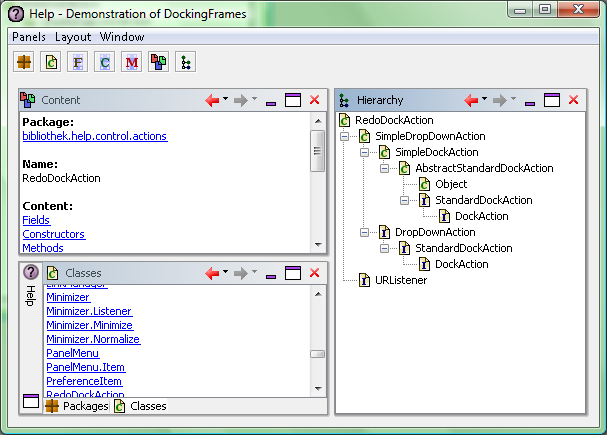
\includegraphics[width=0.5\textwidth]{theme_flat}
\caption{FlatTheme}
\label{fig:theme_basic}
\end{figure}

\subsubsection{BubbleTheme}
A more experimental theme. \src{BubbleTheme} often uses animations and other graphical gimmicks. It has a few performance issues, but it is a good theme to demonstrate the potential of the theme-mechanisms.

\begin{figure}[ht]
\centering
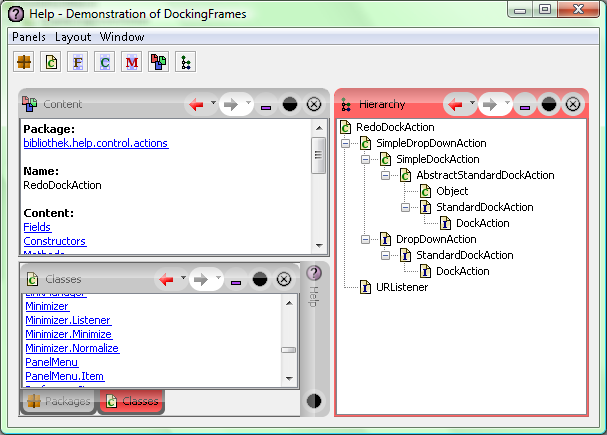
\includegraphics[width=0.5\textwidth]{theme_bubble}
\caption{BubbleTheme}
\label{fig:theme_bubble}
\end{figure}

\subsubsection{EclipseTheme}
\src{EclipseTheme} tries to mimmic the behavior and look of the well known IDE Eclipse. All the \src{Dockable}s are shown on tabbed-components and often \linebreak \src{DockTitle}s are replaced by the tabs. The theme does not use the default theme-mechanisms as often as other themes and it might be a bit tricky to customize the theme. On the other hand it certainly looks good.

\begin{figure}[ht]
\centering
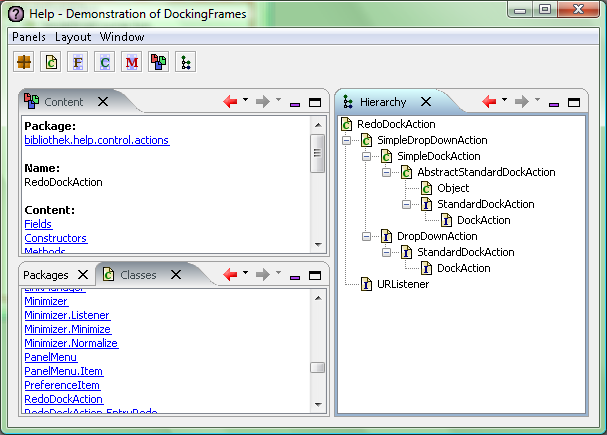
\includegraphics[width=0.5\textwidth]{theme_eclipse}
\caption{EclipseTheme}
\label{fig:theme_eclipse}
\end{figure}

\src{EclipseTheme} offers some keys the map of properties that is stored in \src{DockProperties}. The keys are:
\begin{description}
	\item[PAINT\_ICONS\_WHEN\_DESELECTED] A \src{Boolean} that tells whether \linebreak icons on tabs should be painted if the tab is not selected. In every tabbed-component one tab has to be selected and its associated \src{Dockable} is the only visible element on the component.
	\item[THEME\_CONNECTOR] An \src{EclipseThemeConnector}. The connected tells whether a \src{DockAction} belongs onto a tab, or in a separate list of ``unimportant'' actions. The connector also tells what kind of title to use for a \src{Dockable}.
	\item[TAB\_PAINTER] A \src{TabPainter}. This class is a factory that creates the tab-components and sets up other settings that are related with tabs.
\end{description}

\classbox{The \src{DefaultEclipseThemeConnector} puts every \src{DockAction} which is annotated with \src{EclipseTabDockAction} onto tabs.}

\warningbox{The settings for titles and borders that are given by an \src{EclipseThemeConnector} are not respected if the element is on a \src{StackDockStation}s. A \src{StackDockStation} always uses some tabbed-component.}

\subsection{Customize DockThemes}
More than 50\% of the frameworks source code is only used for painting stuff. No \src{DockTheme} uses particular complex code, just the mass can lead to some loss of direction. This sub-chapter will give only an overview of the basic classes, interfaces and concepts.

\infobox{Many of the mechanisms used by \src{DockTheme}s can be used by clients as well.}

\subsubsection{UI-Properties} \label{sec:uiproperties}
UI-properties is a concept to distribute properties to components. A property could be a \src{Color} and a component some \src{DockTitle} which uses that color to paints it background. The basic idea is to use a map. The keys are \src{String}s, the values are the properties. A \src{DockTheme} or a client can modify or put new key-value pairs into the map and components can read those values which are interesting for them.

Unfortunatelly a simple map is not enough. There needs to be a way to specify values that are used only by a subset of components. Or to remain with the map: the components must become part of the key as well.

The UI-properties provide the necessary features. The mechanism includes these classes, interfaces and generic parameters:
\begin{itemize}
	\item \src{UIProperties}: the base map.
	\item \src{V}: the generic values that have to be distributed, e.g. the class \src{Color}.
	\item \src{UIValue}: A wrapper around \src{V}. Each component creates one \src{UIValue} for each query it will ask the \src{UIProperties}. In example a \src{DockTitle} would have to create and store exactly one \src{UIValue} to represent its background color. \src{UIValue}s also act as observer and the \src{UIProperties} notify an \src{UIValue} if its wrapped \src{V} gets changed.
	\item \src{UIBridge}: An \src{UIBridge} is set between a set of \src{UIValue}s and the \linebreak \src{UIProperties}. \src{V} properties will not be handed directly from \linebreak \src{UIProperties} to \src{UIValue} if there is a bridge between. The bridge can modify the \src{V} property in any way it likes, since the \src{UIBridge} knows the destination of a \src{V} it can also use information derived from the \src{UIValue}.
\end{itemize}

The implementation gets more complex:
\begin{itemize}
	\item For each key several \src{V} properties can be put into the base map. Each value gets assigned another priority (``default'', ``theme'' or ``client'') and only the one with the highest priority is used.
	\item Each \src{UIValue} is associated with a \src{Path}. The \src{Path} tells what an \src{UIValue} will do with the \src{V} property. The \src{Path} also tells what kind of type the \src{UIValue} has.
	\item \src{UIBridge}s are also associated with a \src{Path}. An \src{UIBridge} is responsible to handle all those \src{UIValue}s that are associated either with the same \src{Path} or a \src{Path} that has the bridges \src{Path} as prefix.
\end{itemize}

\designbox{This scheme allows a flexible handling of resources. On one hand the number of keys is limited and one method call is enough to change a lot things in the user interface (e.g. all background colors of titles). On the other hand clients can implement sophisticated strategies to change some properties without the need to know in detail how the property will be used.

Originally this mechanism was invented to handle \src{Color}s. Then it became evident that the same mechanism could be used for other resources as well. The current implementation requires to implement several classes for each type of resource. While this might be annoying for the first use it ensures type safety. In a system where cause (writing in the map) and effect (reading from the map) can be separated by dozens of classes and an unknown amount of time one does not want to care about types as well.}

\subsubsection{Colors}
In order to understand this chapter \ref{sec:uiproperties} should be read first.

All the colors used in the framework are handled by the \src{ColorManager}. The \src{ColorManager} is an \src{UIProperties} and can be accessed through the \linebreak \src{DockController}. It's use could look like this:
\begin{lstlisting}
DockController controller = ...
ColorManager colors = controller.getColors();
colors.put( Priority.CLIENT, "title.active.left", Color.GREEN );
\end{lstlisting}
In this snippet the value for the key ``title.active.left'' is changed to green. The priority \src{CLIENT} is highest possible priority. It is never overridden by the framework.

Or a more sophisticated use could involve a \src{ColorBridge}:
\begin{lstlisting}
DockController controller = ...
ColorManager colors = controller.getColors();
colors.publish( Priority.CLIENT, TitleColor.KIND_TITLE_COLOR, new ColorBridge(){
	public void add( String id, DockColor uiValue ){
		// ignore
	}
	public void remove( String id, DockColor uiValue ){
		// ignore
	}
	public void set( String id, Color value, DockColor uiValue ){
		TitleColor title = (TitleColor)uiValue;
		if( title.getTitle().getDockable() == <somevalue> )
			title.set( Color.GREEN );
		else
			title.set( value );
	}	
});
\end{lstlisting}
Here a \src{ColorBridge} for the \src{Path} \src{KIND\_TITLE\_COLOR} is installed in line \src{3}. This path is only used by \src{UIValue}s that implement \src{TitleColor}. Hence the unchecked cast from \src{DockColor} to \src{TitleColor} in line \src{11} is safe. The methods \src{add} (line \src{4-6}) and \src{remove} (line \src{7-9}) are called by \src{UIProperties} when a \src{UIValue} gets added or removed to it. These methods can be ignored as long as the bridge does not change the color on its own. Otherwise the \src{DockColor}s could be stored in some list and their method \src{set} could be called whenever the color needs to be exchanged.

This bridge searches for a specific \src{Dockable} called ``somevalue'' (line \src{12}). The bridge returns \src{GREEN} for all colors used by any title of this \src{Dockable}. There is no distinction between the colors for background, foreground or other usages.

\infobox{There is no global list of keys and every \src{DockTheme} uses different keys. All the modules that need colors are annotated with \src{ColorCodes} and expose their own list of keys to the API-documentation. Also the method \src{updateColors} of \src{BasicTheme} or subclasses can help: in this method all the colors that will ever be used by the theme are written into the \src{ColorManager}.}

\classbox{All the standard themes use a \src{ColorScheme} as their initial set of colors. All the standard themes provide a key for the \src{DockProperties} to change that initial scheme. For example the key provided by \src{BasicTheme} is stored as constant \src{BASIC\_COLOR\_SCHEME}. There are several subclasses of \src{ColorScheme} for the different themes.}

By the way: some themes use colors that are read from the current \linebreak \src{LookAndFeel}. Clients can call the method \src{registerColors} of \src{DockUI}. This method takes a \src{LookAndFeelColors} which is responsible in reading the colors from the \src{LookAndFeel}.

\subsubsection{Fonts}
Fonts use the same mechanism as Colors. A \src{FontManager} can be accessed through the methods \src{getFonts} of \src{DockController}. Unlike colors a set of standard keys are defined as constants in \src{DockFont}.

The \src{FontManager} does not distribute \src{Font}-objects but \src{FontModifier}s. A \src{FontModifier} has one method that receives the original \src{Font} and can return any \src{Font} it likes. In example a \src{FontModifier} could inverse the bold-property of a \src{Font}. There are two \src{FontModifiers} ready to use:
\begin{itemize}
	\item \src{ConstantFontModifier} does not modify anything but always return the same \src{Font}
	\item \src{GenericFontModifier} can modify the italic-, bold- and size-property of a font.
\end{itemize}

\classbox{Clients that want to use a \src{FontModifier} might be interested in the classes \src{DLabel} and \src{DPanel} which already modify their font. Also the class \src{FontUpdater} can be used to create new \src{JComponent}s with the capability to modify their font.}

\subsubsection{Icons}
\src{Icon}s can be modified through the \src{IconManager}. The \src{IconManager} is just a map with the capability to inform observers if some of its value changed. The \src{IconManager} can be accessed through the method \src{getIcons} of \linebreak \src{DockController}.

There is no global list of keys in the source code. However the file ``icons.ini'' contains a list of keys and paths of all the default icons.

\subsubsection{Actions}
The views for \src{DockAction}s are changed through the \src{ActionViewConverter}. Please read chapter \ref{sec:actions} for more information.

\subsubsection{Titles}
\src{DockTitle}s are managed by the \src{DockTitleManager}. Please read chapter \ref{sec:titles} for more information.

\subsection{Custom Theme}
With the exception of the classes that are directly related to a \src{DockTheme} no code in the framework depends on a special undocummented behavior of a theme. Clients can reimplement the interface \src{DockTheme} without fear to break things.

A better approach then full reimplementation might be to extend the class \src{BasicTheme}. This class provides some default values which can easily be \linebreak changed by the appropriate \src{setXZY} method.

\src{DockTheme} has a method \src{install}, this method can be used to exchange some values that are not stored in the \src{DockTheme} itself. For example to exchange icons in the \src{IconManager}.

\warningbox{A theme dives deep into the framework. Implementing a new theme requires a lot of time and a good understanding of the framework. This document might help to understand the basics, but some stuff can only be found out by looking directly at the source code.}

\section{Drag and Drop}
To drag a \src{Dockable} to a new location and drop it there is the most important feature of any docking framework. Surprisingly the implementation of this part is very small.

\subsection{Relocator}
The sourcecode that detects drag gestures, searches for the target station and makes sure that the user has some visual feedback is located in the \linebreak \src{DefaultDockRelocator}. \src{DefaultDockRelocator} itself extends from \linebreak \src{DockRelocator} which just allows to register some listeners and set some useful properties. Clients seldomly need to implement a new \src{DockRelocator}. If they do, then they have to implement a new \src{DockControllerFactory}. The code will look like this:

\begin{lstlisting}
public class MyDockControllerFactory extends DefaultDockControllerFactory{
  @Override
  public DockRelocator createRelocator( DockController controller ) {
    return new MyDockReloactor();
  }
}
\end{lstlisting}
This factory has then to be given to the constructor of a \src{DockController}. For the remainder of this chapter it is assumed, that the default relocator is in use.

The \src{DockRelocator} that is in use can be accessed through the method \src{getRelocator} of \src{DockController}.

\subsection{Sources}
The relocator needs to know where and when the user presses and moves the mouse. There is more than one solution for this problem.

\subsubsection{DockElementRepresentative}
A \src{DockElementRepresentative} is a \src{Component} which represents a \src{Dockable}. Anyone can add \src{MouseInputListener}s to a representative and hence be informed about anything the mouse does on top of such a \src{Component}.

\src{DockTitle} and \src{Dockable} are two implementations of \linebreak \src{DockElementRepresentative}. Their registration is handled automatically. If clients implement a new representative then they should call the methods \linebreak \src{addRepresentative} and \src{removeRepresentative} of \src{DockController} to install or uninstall the representative.

\infobox{\src{DockElementRepresentative} was added late to the framework. It carries some legacy code: the method \src{isUsedAsTitle}. This method introduces a distinction between those representations for which all features are activated (e.g. popup menus) and those for which only a selected subset is available. Normally clients implement representatives that are used as title and can return \src{true} here.}

\warningbox{The behavior for representations of \src{Dockable}s that are not registered is unspecified. Clients should not add a \src{DockElementRepresentative} if its \src{Dockable} is unknown to the \src{DockController}.}

\subsubsection{Remote control}
Sometimes it is not possible to implement a \src{DockElementRepresentative}. Remote control of a relocator is an alternative for these cases. Remote control is realized by the classes \src{RemoteRelocator} and \src{DirectRemoteRelocator}.

A \src{RemoteRelocator} can be optained by calling \src{createRemote} of \linebreak \src{DockRelocator}. \src{RemoteRelocator} should be used in combination with a \linebreak \src{MouseListener} and a \src{MouseMotionListener}:
\begin{itemize}
 \item \src{MouseListener.mousePressed} \textrightarrow \src{RemoteRelocator.init}
 \item \src{MouseMotionListener.mouseDragged} \textrightarrow \src{RemoteRelocator.drag}
 \item \src{MouseListener.mouseReleased} \textrightarrow \src{RemoteRelocator.drop}
\end{itemize}
The methods \src{init}, \src{drag} and \src{drop} return a \src{Reaction}. The reaction tells the caller what to do next:
\begin{itemize}
 \item \src{CONTINUE}: the operation continues, the event was ignored.
 \item \src{CONTINUE\_CONSUMED}: the operation continues, the event was consumed. The caller should invoke \src{MouseEvent.consume}.
 \item \src{BREAK}: the operation was canceled, the event was ignored.
 \item \src{BREAK\_CONSUMED}: the operation was canceled, the event was consumed. The caller should invoke \src{MouseEvent.consume}.
\end{itemize}

A \src{DirectRemoteRelocator} can be optained by calling \src{createDirectRemote} of \src{DockRelocator}. A \src{DirectRemoteRelocator} is basically the same as a \src{RemoteRelocator} but always assumes that the user pressed the correct button on the mouse. Its methods do not return a \src{Reaction} because it would always be the same.

\infobox{Clients can use several remote controls at the same time, they will cancel out each other if necessary. A \src{RemoteRelocator} can be used several times.}

\subsection{Destinations}
A relocator needs to find the one \src{DockStation} on which the \src{Dockable} is dropped. 

\subsubsection{Search}
The \src{DefaultDockRelocator} searches the destination anew whenever the mouse is moved. The search includes these steps:
\begin{enumerate}
 \item An ordered list of all potential destinations is built. A \src{DockStation} is a potential destination if it is visible (\src{isStationVisible} of \src{DockStation}), not the dragged \src{Dockable} nor one of its children, and its boundaries contain the location of the mouse (\src{getStationBounds} of \src{DockStation}). The order depends on parent-child relations between the stations, between the \src{Window}s on which the stations are, and on custom conditions that every station can offer (\src{canCompare} and \src{compare} of \src{DockStation}).
 \item Then the method \src{prepareMove} or \src{prepareDrop} of \src{DockStation} is called. These methods check whether the station really is a good destination. They return \src{true} if so, \src{false} if not. The first station that returns \src{true} is the destination.
 \item The method \src{draw} of the new destination is called, the method \src{forget} on the old destination. The new destination will paint some markings to give a visual feedback to the user, the old destination will delete all the information about any drag and drop operation.
\end{enumerate}

\classbox{There is more information about the exact semantics in the API-documentation for \src{DockStation}.}

\designbox{Due of the varieties of stations a general interface for drag and drop would be very hard to come up with. Hence most of the work has to be done by the stations itself. This might lead to code that is written twice, but also allows much freedom in writing stations. There are some helper classes that can help with the most common tasks:
\begin{itemize}
 \item \src{DockController.getAcceptance} to access all the global acceptance tests at once.
 \item \src{StationPaint}, accessible through \src{DockUI.getPaint}.
\end{itemize}

}

\subsubsection{Drop}
The moment a user releases the mouse and drops a \src{Dockable} the method \src{move} or \src{drop} of \src{DockStation} is called. These methods can either put the \src{Dockable} somewhere onto the station or merge the \src{Dockable} with an existing child of the station (sometimes referred as ``put'' and ``merge'' action). The results of the first reaction depend on the kind of station. The results of the second reaction are independent of the kind of station.

Merging normally results in creating a new \src{StackDockStation}. The existing child and the dropped \src{Dockable} are put onto that new station. Then the \src{StackDockStation} is put at the place where the existing child was. Creation of ``merged \src{Dockable}s'' is handled by a \src{Combiner}, per default by the \src{BasicCombiner}. Many \src{DockStation}s have a method that allows clients to set their own implementation of a \src{Combiner}. Clients can exchange the \src{Combiner} globally by creating a new \src{DockTheme}, overriding the method \src{getCombiner} and then registering a new instance at the \src{DockController} through \src{setTheme}. Note that all descendants of \src{BasicDockTheme} have a method called \src{setCombiner} that exchanges the \src{Combiner} directly without the need to override \src{getCombiner}.

\warningbox{Exchanging a \src{Combiner} does not affect any existing \src{Dockable} or \src{DockStation}, it will only affect the creation of new elements.}

\subsection{Influences}
There are a number of factors that can influence the search for a new destination. Some of them are customizable.

\subsubsection{Modes}
A \src{DockRelocator} can have "modes". A mode is some kind of behavior that is activated when the user presses a certain combination of keys. Modes are modeled by the class \src{DockRelocatorMode}. It is not specified what effect a mode really has, but normally a mode would add some restrictions where to put a \src{Dockable} during drag and drop. \src{DockRelocatorMode}s can be added or removed to a \src{DockRelocator} by the methods \src{addMode} and \src{removeMode}.

Currently two modes are installed:
\begin{description}
\item[DockRelocatorMode.SCREEN\_ONLY] (press key \textit{shift}) ensures that a \linebreak \src{Dockable} can only be put on a \src{ScreenDockStation}. That means that a \src{Dockable} can be directly above a \src{DockStation} like a \src{SplitDockStation}, but can't be dropped there.
\item[DockRelocatorMode.NO\_COMBINATION] (press key \textit{alt}) ensures that a \src{Dockable} can't be put over another \src{Dockable}. That means, every operation that would result in a merge is forbidden. Also dropping a \src{Dockable} on already merged \src{Dockable}s will not be allowed.
\end{description}

\classbox{The keys that have to be pressed to activate \src{SCREEN\_ONLY} or \src{NO\_COMBINATION} are the properties \src{SCREEN\_MASK} and \src{NO\_COMBINATION\_MASK}. The can be changed by accessing the \src{DockProperties}.}

\subsubsection{Restrictions}
The set of possible destinations for a \src{Dockable} can be restricted. There are several reasons why a client or the framework itself would do that:
\begin{itemize}
 \item Some \src{Dockable} must always be visible.
 \item Some \src{DockStation}s represent a special area that can only be used by a subset of \src{Dockable}s.
 \item Some \src{Dockable}s can only be presented on a certain kind of \src{DockStation}.
\end{itemize}

These restrictions are implemented through acceptance tests. An acceptance test either checks one ``put'' or one ``merge'' action. Tests can be stored at various locations:
\begin{itemize}
 \item Every \src{Dockable} has two methods called \src{accept}.
 \item Each \src{DockStation} has a method \src{accept}. This method tells whether some \src{Dockable} can become a child of the \src{DockStation}. This method checks ``put'' and ``merge'' actions at the same time.
 \item And then there are \src{DockAcceptance}s. A \src{DockAcceptance} has \src{accept}-methods too. These methods get a \src{DockStation} and some \src{Dockable}s, and then have to decide whether the elements can be put together. Each \src{DockAcceptance} works on a global scale, and thus they are registered at the \src{DockController} through \src{addAcceptance}.
\end{itemize}

\warningbox{Acceptance tests are very powerful. They have to be implemented carefully or the drag and drop mechanism might become crippled.}

\designbox{Acceptance tests are performed by the potential destination \src{DockStation}. The \src{DockStation} is the first module that knows where a \src{Dockable} will land. Handling acceptance tests allows the station to cut down the amount of work it does, and to try alternative actions (e.g. a ``put'' instead of a ``merge'' action) if some future configuration does not pass the tests.

The drawback is, that a \src{DockStation} can break the mechanism by just not performing the tests.}

\section{Preferences}
The preference system allows the user to change settings which are otherwise not accessible. An example would be the shortcut for maximizing a \src{Dockable} (\src{ctrl+m}). The preference system makes a sharp distinction between model and view, clients are free to integrate the model in their own view, or to create a new model and using the standard view. Figure \ref{fig:preferences} shows the simple version of the standard view with some random preferences.

\begin{figure}[ht]
\centering
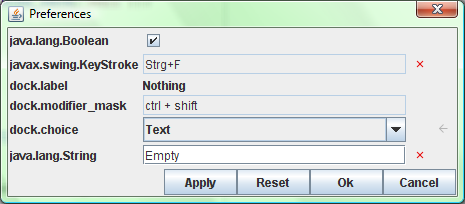
\includegraphics[width=0.5\textwidth]{preferences}
\caption{The \src{PreferenceDialog} showing some random preferences.}
\label{fig:preferences}
\end{figure}

\subsection{Model}
This section explains how the model is organized.

\subsubsection{Preference}
A preference is an abstract concept. One preference represents some property of the framework (or of the client). A preference is a set of meta-informations about a property:
\begin{description}
 \item[Path] A unique identifier
 \item[TypePath] Tells how to work with \src{Value}. For example how to present the value to the user (as text, as image...) or how to store the value. An object of type \src{Path} is used to represent the \src{TypePath}.
 \item[Value] The current value of the property.
 \item[ValueInfo] Information about the value, e.g. the maximum value for an \linebreak \src{Integer}-property. The exact meaning of this information depends on the \src{TypePath}.
\end{description}

\designbox{\src{Value} is some \src{Object} and \src{TypePath} tells the view how to cast \src{Value} in order to use it. If \src{TypePath} were a \src{Class} then there would never be doubt whether the correct cast is performed. But \src{TypePath} is a \src{Path} and hence an additional indirection is introduced.

The reason for this is that the same \src{Object} might need different treatment in different situations. E.g. an \src{Integer} could just be an int, it could be a natural number or it could be an int from the range 1 to 100.}

\classbox{There is an interface \src{Preference} and a class \src{DefaultPreference} which bring this preference-abstraction to code. It is not necessary to use them, they are just here to simplify things.}

\subsubsection{PreferenceModel}
The \src{PreferenceModel} is the basic module of the preference system. A \linebreak \src{PreferenceModel} is a list of preferences (the abstraction, not the interface). It often acts as mediator between some unspecified storage mechanism for properties and the user interface. The methods \src{read} and \src{write} are used to access that covered storage mechanism. To transfer values into the model \src{read} is called, to transver values to the storage mechanism \src{write} is called.

\classbox{\src{DefaultPreferenceModel} is the standard implementation of \src{PreferenceModel}. Its entries are objects of type \src{Preference}.

Several models can be combined using a \src{MergedPreferenceModel}.}

\infobox{There are several subclasses of \src{DefaultPreferenceModel} for various settings that can be made. For example \src{EclipseThemeModel} handles properties of \src{EclipseTheme}.

There are also many implementations of \src{Preference} for various properties of the framework. The API-documentation reveals more.}

\subsubsection{PreferenceTreeModel}
This model is a \src{PreferenceModel} and a \src{javax.swing.TreeModel}. If seen as \src{PreferenceModel}, then it behaves like a \src{MergedPreferenceModel}. If seen as \src{TreeModel}, then it contains \src{PrefereceTreeModel.Node}-objects. A node can either be just a name, or another \src{PreferenceModel}. This model is intended to be used in a \src{JTree} where the user can select one aspect of the whole set of preferences to show.

\classbox{The subclass \src{DockingFramesPreferenceModel} is the set of preferences which includes all the aspects of the core-library.}

\subsection{View}
A \src{PreferenceModel} is best displayed in a \src{PreferenceTable}. This table will show a label, an editor and operations for each preference. 

A \src{PreferenceTreeModel} can be displayed in a \src{PreferenceTreePanel}. It will show not only a \src{PreferenceTable} but also a \src{JTree} where the user can select which sub-model to edit.

Further more the \src{PreferenceDialog} and the \src{PreferenceTreeDialog} are available. These dialogs offer the options to apply the settings, to cancel editing and to reset all preferences to their default value.

\subsubsection{Editors}
Since there are different types of preferences, different editors are needed. The kind of editor for one preference is determined by the type-path (\src{getTypePath} in a model). Clients can add new editors to a \src{PreferenceTable} through the method \src{setEditorFactory}.

An editor is always of type \src{PreferenceEditor}. Each editor gets a \linebreak \src{PreferenceEditorCallback} with which it can interact with the table. Whenever the user changes the editors value, the editor should call the method \src{set} of \src{PreferenceEditorCallback} to make sure the new value gets stored.

\subsubsection{Operations}
There are some operations which should be available for almost any preference. For example \textit{set a default value} or \textit{delete the current value}. The preference system introduces the \src{PreferenceOperation} to handle these kind of actions.

A \src{PreferenceOperation} is nothing more than a label and an icon. The logic for an operation is either in an editor or in a model.

\begin{description}
 \item[Editor:] Editors with operations must call the method \src{setOperation} of \linebreak \src{PreferenceEditorCallback} for each operation they offer. By calling \src{setOperation} more than once, the editor can change the enabled state of the operation. If the user triggers an operation of the editor, the method \src{doOperation} of \src{PreferenceEditor} is called. It is then the editors responsibility to handle the operation.
 \item[Preference:] Preferences can have operations as well. The method \linebreak \src{getOperations} of \src{PreferenceModel} will be called once to get all the available operations for one preference. The method \src{isEnabled} will be invoked to find out whether an operation is enabled or not. Models can change the enabled state by calling \src{preferenceChanged} of \linebreak \src{PreferenceModelListener}. If the user triggers an operation, \linebreak \src{doOperation} of \src{PreferenceModel} will be invoked.
\end{description}
If an editor and a preference share the same operations, then per definition the operations belong to the editor. All settings from the model will just be ignored.

\infobox{Operations might be confusing at first, but they can be really useful. The strength of operations is that they are handled automatically, and that they need not much code.}

\subsection{Storage}
The \src{PreferenceStorage} can be used to store \src{PreferenceModel}s in memory or persistent either as byte-stream or as XML.

The normal way to write a model from memory to the disk looks like this:
\begin{lstlisting}
// the stream we want to write into
DataOutputStream out = ...

// the model we want to store
PreferenceModel model = ...

// And now store the model
PreferenceStorage storage = new PreferenceStorage();
storage.store( model );
storage.write( out );
\end{lstlisting}
Note that there are two phases in writing \src{model}. First the model gets \src{store}d (line \src{9}) into \src{storage}. It is possible to store more than just one model in a \src{PreferenceStorage}. Second \src{storage} gets written onto the disk in line \src{10}.

The standard way to read a model are to apply the same steps in reverse:
\begin{lstlisting}
// the source of any new data
DataInputStream in = ...

// the model we want to load
PreferenceModel model = ...

// And now load the model
PreferenceStorage storage = new PreferenceStorage();
storage.read( in );
storage.load( model, false );
\end{lstlisting}
Like writing this operation has two phases. In line \src{9} \src{storage} gets filled with information, in line \src{10} the information gets transfered to \src{model}. The argument \src{false} is a hint what to do with missing preferences. In this case missing preferences are just ignored. A value of \src{true} would force them to become \src{null}.

There are some preferences which do not need to be stored by the \linebreak \src{PreferenceStorage} because they are already stored by the underlying system. These preferences are called \textit{natural}, while the others are called \textit{artificial}. The method \src{isNatural} of \src{PreferenceModel} can be used to distinguish them.

\designbox{The distinction between natural and artificial preferences might seem curious. But actually this allows to use an unlimited number of storage mechanisms at the same time.}

\subsection{Lifecycle}
This section describes the best way how to use a \src{PreferenceModel}.

The correct lifecycle of a \src{PreferenceModel} includes normally these steps:
\begin{enumerate}
 \item Create the model. Set up all the preferences that are used by the model.
 \item Call \src{load} on a \src{StoragePreference}.
 \item Call \src{write} on the model to synchronize the model with the underlying system.
 \item (work with the underlying system)
 \item To work with the model: call first \src{read}, then make the changes in the model, then call \src{write}.
 \item (work with the underlying system)
 \item Call \src{read} on the model to synchronize the model with the underlying system.
 \item Store the model using \src{store} of a \src{PreferenceStorage}.
\end{enumerate}

If the \src{PreferenceStorage} used in step \src{2} is empty because its \src{read} or \src{readXML} method failed, then calling \src{read} of \src{PreferenceModel} would at least load some default settings.

Steps \src{4, 5, 6} can be cycled as many times as needed.

An additional step \src{0} and \src{9} would be to read and write the \\\src{PreferenceStorage} when starting up or shuting down the application.

\section{Properties}
There are a number of interesting settings whose effects are deeply hidden within the framework. Properties are an easy way to access these settings and change them. Properties are represented by the class \src{DockProperties} which can be accessed through \src{getProperties} of \src{DockController}.

\src{DockProperties} is nothing else than a map. As keys are instances of \src{PropertyKey} used. The type of the value depends on the key and the map is typesafe. With the help of a \src{DockPropertyListener} any object can be informed immediately when a value changes.

There are a number of keys and the remainder of this chapter will list all of the keys that are present in version 1.0.7. If not explicitly said otherwise, then any change in the properties will have an immediate effect.

\warningbox{Some of these properties are accessed and changed by \src{DockTheme}s.}

\subsection{Themes}
\begin{description}
 \property{BasicTheme.BASIC\_COLOR\_SCHEME}{ColorScheme}{An instance of \src{BasicColorScheme}}{The \src{ColorScheme} used by \src{BasicTheme}.}
 \property{BubbleTheme.BUBBLE\_COLOR\_SCHEME}{ColorScheme}{An instance of \src{BubbleColorScheme}}{The \src{ColorScheme} used by \src{BubbleTheme}.}
 \property{FlatTheme.FLAT\_COLOR\_SCHEME}{ColorScheme}{An instance of \src{FlatColorScheme}}{The \src{ColorScheme} used by \src{FlatTheme}.}
 \property{EclipseTheme.ECLIPSE\_COLOR\_SCHEME}{ColorScheme}{An instance of \src{EclipseColorScheme}}{The \src{ColorScheme} used by \src{EclipseTheme}.}
 \property{EclipseTheme.PAINT\_ICONS\_WHEN\_DESELECTED}{Boolean}{\src{false}}{Whether to paint icons in tabs of \src{Dockable}s that are not selected. This setting might be ignored if a custom \src{TabPainter} is applied.}
 \property{EclipseTheme.TAB\_PAINTER}{TabPainter}{\src{ShapedGradientPainter.FACTORY}}{How to paint tabs in \src{EclipseTheme} for \src{Dockable}s.}
 \property{EclipseTheme.THEME\_CONNECTOR}{EclipseThemeConnector}{An instance of \src{DefaultEclipseThemeConnector}}{Tells how a lonly \src{Dockable} gets presented in \src{EclipseTheme}. \linebreak Whether it has a border and a title. Also tells which \src{DockAction}s are to be shown on tabs. Changing this entry will not affect decisions that were made by the previous connector.}
\end{description}

\subsection{Stations}
\begin{description}
 \property{FlapDockStation.LAYOUT\_MANAGER}{FlapLayoutManager}{An instance of \src{DefaultFlapLayoutManager}}{Tells the initial size and whether to hold a \src{Dockable} in a \linebreak \src{FlapDockStation}. The default setting uses the same size for all \src{Dockable}s and forgets the hold-property as soon as a \src{Dockable} is removed from the station.}
 \property{FlapDockStation.BUTTON\_CONTENT}{ButtonContent}{\src{ButtonContent.THEME\_DEPENDENT}}{Tells which information to display on the buttons that represent \src{Dockable}s on a \src{FlapDockStation}. Any mix of icons, text and \src{DockAction}s is possible.}
 \property{ScreenDockStation.BOUNDARY\_RESTRICTION}{BoundaryRestriction}{\src{BoundaryRestriction.FREE}}{Decides about the shape and location a \src{ScreenDockWindow} is allowed to have. E.g. \src{BoundaryRestriction} might force windows to be visible only on one of many screens.}
 \property{ScreenDockStation.WINDOW\_FACTORY}{ScreenDockWindowFactory}{An instance of \src{DefaultScreenDockWindowFactory}}{The factory used to create new windows for \src{ScreenDockStation}. Changing this property has no effect on existing windows. \linebreak \src{DefaultScreenDockWindowFactory} can be customized and should be preferred over newly written factories.}
 \property{StackDockStation.COMPONENT\_FACTORY}{StackDockComponentFactory}{\src{null}}{Tells a \src{StackDockStation} how to arrange its children.}
 \property{SplitDockStation.MAXIMIZE\_ACCELERATOR}{KeyStroke}{\src{ctrl+m}}{The keys that have to be pressed in order to maximize or normalize a child of \src{SplitDockStation}.}
 \property{SplitDockStation.LAYOUT\_MANAGER}{SplitLayoutManager}{An instance of \src{DefaultSplitLayoutManager}}{The \src{SplitLayoutManager} is responsible to handle most of the actions that can change the layout of a \src{SplitDockStation}}
\end{description}

\subsection{Controlling}
\begin{description}
 \property{DockableSelector.INIT\_SELECTION}{KeyStroke}{\src{ctrl+shift+e}}{Hitting these keys will open a window where the user can select the focused \src{Dockable}.}
 \property{DockRelocatorMode.SCREEN\_MASK}{ModifierMask}{\src{shift}}{If these modifiers are pressed during a drag and drop operation then \src{DockRelocatorMode.SCREEN\_ONLY} gets activated. This will \linebreak force the \src{Dockable} to be dropped onto a \src{ScreenDockStation}.}
 \property{DockRelocatorMode.NO\_COMBINATION\_MASK}{ModifierMask}{\src{alt}}{If these modifiers are pressed during a drag and drop operation then \src{DockRelocatorMode.NO\_COMBINATION} gets activated. This will prevent the dropped \src{Dockable} from merging with another \src{Dockable}.}
 \property{DockFrontend.HIDE\_ACCELERATOR}{KeyStroke}{\src{ctrl+F4}}{If a \src{DockFrontend} is in use then hitting these keys will hide the currently focused \src{Dockable}.}
\end{description}
 
\subsection{Legacy}
\begin{description}
 \property{AWTComponentCaptureStrategy.STRATEGY}{AWTComponentCaptureStrategy}{\src{PAINT\_ALL\_STRATEGY}}{Tells how the framework can take a picture from a \src{Component} that is or contains an AWT-\src{Component}. Different strategies are available, some are more subtile but efficient, others are blunt but working under harsh conditions.}
\end{description}

\subsection{Gimmicks}
\begin{description}
 \property{PropertyKey.DOCKABLE\_ICON}{Icon}{\src{null}}{This icon is shown for any \src{Dockable} that has no icon set.}
 \property{PropertyKey.DOCKABLE\_TITLE}{String}{\src{null}}{This text is shown for any \src{Dockable} that has no title set.}
 \property{PropertyKey.DOCKABLE\_TOOLTIP}{String}{\src{null}}{This text is shown for any \src{Dockable} for which no tooltip was set.}
 \property{PropertyKey.DOCK\_STATION\_ICON}{Icon}{\src{null}}{This icon is shown for any \src{DockStation} that has no icon set.}
 \property{PropertyKey.DOCK\_STATION\_TITLE}{String}{\src{null}}{This text is shown for any \src{DockStation} that has no title set.}
 \property{PropertyKey.DOCK\_STATION\_TOOLTIP}{String}{\src{null}}{This text is shown for any \src{DockStation} for which no tooltip was set. }
\end{description}

\end{document} 